\documentclass[a4paper, 12pt]{article}

\usepackage[portuges]{babel}
\usepackage[utf8]{inputenc}
\usepackage{amsmath}
\usepackage{indentfirst}
\usepackage{blindtext}
\usepackage{graphicx}
\usepackage[hidelinks]{hyperref}
\usepackage{gensymb}

\author{Igor Abreu da Silva}

\title{Trabalho Final de Sistemas Lineares I}

\begin{document}
	
	\begin{titlepage}
		\begin{center}
			\huge{Universidade Federal do Rio de Janeiro}
			\vspace{95pt}
			
			\large{Lista I - Sistemas Lineares I}
			\vspace{160pt}
		\end{center}
		
		\begin{flushleft}
			\begin{tabbing}
				Alunos\qquad\qquad\= Igor Abreu da Silva\\
				DRE\> 112053874 \\
				Curso\> Engenharia Eletrônica \\
				Turma\> 2016/2 \\
				Professor\> Natanael Nunes de Moura Junior \\
				
			\end{tabbing}
			
		\end{flushleft}
		
		\begin{center}
			\vspace{\fill}
			Rio de Janeiro, 16 de Setembro de 2016
		\end{center}
	\end{titlepage}
	
	\newpage
	\tableofcontents
	\listoffigures
	\thispagestyle{empty}
	\newpage
	\pagenumbering{arabic}
	
	\section{Quest\~{a}o 1 - Conhecimentos Básicos}
		\subsection{Item a}	
			\begin{figure}[!ht]
				\centering
				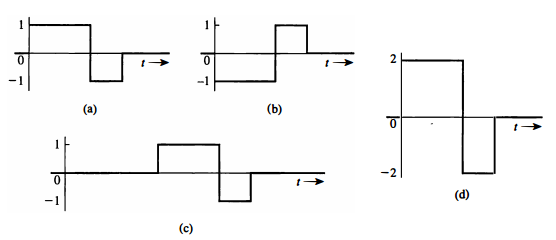
\includegraphics{img/Figura1.png}
				\caption{Sinais utilizados no Item A}	
			\end{figure}
			Analisando os resultados, percebe-se que a inversão ou o deslocamento não alteram a energia do sinal, entretanto, a multiplicação por um fator k altera o sinal em $k^{2}$.
			\subsubsection{Sinal (a)}
			$\int_{0}^{2} 1^{2}dx + \int_{2}^{3} -1^{2}dx \Rightarrow  \int_{0}^{2}dx + \int_{2}^{3}dx = 3$ 
			\subsubsection{Sinal (b)}
			$\int_{0}^{2} -1^{2}dx + \int_{2}^{3} 1^{2}dx \Rightarrow  \int_{0}^{2}dx + \int_{2}^{3}dx = 3$ 	
			\subsubsection{Sinal (c)}
			$\int_{3}^{5} 1^{2}dx + \int_{5}^{6} -1^{2}dx \Rightarrow  \int_{3}^{5}dx + \int_{5}^{5}dx = 3$ 		
			\subsubsection{Sinal (d)}
			$\int_{0}^{2} 2^{2}dx + \int_{2}^{3} -2^{2}dx \Rightarrow  \int_{0}^{2}4dx + \int_{2}^{3}4dx = 12$ 	
			\newpage	
		\subsection{Item b}	
			\begin{figure}[!ht]
				\centering
				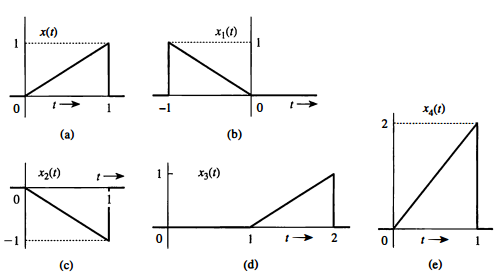
\includegraphics{img/Figura2.png}
				\caption{Sinais utilizados no Item B}	
			\end{figure}		
			Repete-se o que ocorre no Item(a)
			\subsubsection{Sinal (a)}
			$\int_{0}^{1} x^{2}dx  = \frac{1}{3}$
			\subsubsection{Sinal (b)}
			$\int_{-1}^{0} (-x)^{2}dx  = \frac{1}{3}$ 
			\subsubsection{Sinal (c)}
			$\int_{0}^{1} (-x)^{2}dx  = \frac{1}{3}$				
			\subsubsection{Sinal (d)}
			$\int_{1}^{2} (x-1)^{2}dx  \Rightarrow \int_{1}^{2} (x^{2}-2x+1)dx = \frac{8}{3} - \frac{1}{3} - 4 +1 + 2 -1 = \frac{1}{3}$ 		
			\subsubsection{Sinal (e)}
			$\int_{0}^{1} (2x)^{2}dx  = \frac{4}{3}$ 					
		\subsection{Item c}	
			\begin{figure}[!ht]
				\centering
				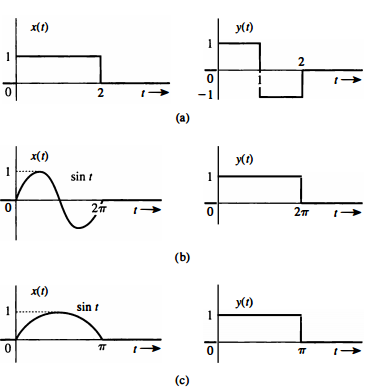
\includegraphics{img/Figura3.png}
				\caption{Sinais utilizados no Item C}	
			\end{figure}		
			\subsubsection{Sinais (a)}
			\[E_{x} = \int_{0}^{2} 1^{2}dx = 2 \]
			\[E_{y} = \int_{0}^{1} 1^{2}dx + \int_{1}^{2} -1^{2}dx \Rightarrow 1 + 1 = 2 \]
			\[E_{x+y} = \int_{0}^{1} 2^{2}dx = 4 \]
			\[E_{x-y} = \int_{1}^{2} -2^{2}dx = 4 \]	
			\subsubsection{Sinais (b)}
			\[E_{x} = \int_{0}^{2\pi} sin^{2}(x)dx \Rightarrow \int_{0}^{2\pi} \frac{1-cos(2x)}{2} \Rightarrow  \frac{1}{2}\int_{0}^{2\pi} 1dx - \frac{1}{2}\int_{0}^{2\pi} cos(2x)dx = \pi + 0 = \pi\]
			\[E_{y} = \int_{0}^{2\pi} 1^{2}dx  = 2\pi \]
			\[E_{x+y} = \int_{0}^{2\pi} (sin(x) +1)^{2}dx \Rightarrow \int_{0}^{2\pi} \frac{1-cos(2x)}{2} + 2sen(x) + 1\Rightarrow\]\[ \frac{1}{2}\int_{0}^{2\pi} 1dx - \frac{1}{2}\int_{0}^{2\pi} cos(2x)dx + 2\int_{0}^{2\pi} sin(x)dx + \int_{0}^{2\pi} 1dx= \pi + 0 + 0 + 2\pi = \pi\]
			\[E_{x-y} = \int_{1}^{2} -2^{2}dx = 4 \]							
		\subsection{Item d}	
		\subsection{Item e}	
		\subsection{Item f}	
		\subsection{Item g}	
		\subsection{Item h}	
		\subsection{Item i}	
		\subsection{Item j}	
		\subsection{Item k}	
		\subsection{Item l}	
		\subsection{Item m}	
		\subsection{Item n}		
	\section{Quest\~{a}o 2 - Conhecimentos Básicos}
		\subsection{Item a}	
		\subsection{Item b}	
		\subsection{Item c}	
		\subsection{Item d}	
		\subsection{Item e}	
		\subsection{Item f}	
		\subsection{Item g}	
		\subsection{Item h}	
	\section{Quest\~{a}o 3 - Conhecimentos Básicos}
		\subsection{Item a}	
		\subsection{Item b}	
		\subsection{Item c}	
		\subsection{Item d}	
		\subsection{Item e}	
	\section{Quest\~{a}o 4 - Conhecimentos Básicos}
		\subsection{Item a}	
		\subsection{Item b}	
		\subsection{Item c}	
	\section{Quest\~{a}o 5 - Classificação de Sinais}		
	\section{Quest\~{a}o 6 - Classificação de Sistemas}			
		\subsection{Item a}	
		\subsection{Item b}	
		\subsection{Item c}		
	\section{Quest\~{a}o 7 - Classificação de Sistemas}			
		\subsection{Item a}	
		\subsection{Item b}			
	\section{Quest\~{a}o 8 - Energia e Potência de Sinais}	
	\section{Quest\~{a}o 9 - Operação com Sinais}
		\subsection{Item a}	
		\subsection{Item b}	
		\subsection{Item c}	
		\subsection{Item d}		
	\section{Quest\~{a}o 10 - Operação com Sinais}
		\subsection{Item a}	
		\subsection{Item b}					
		


		

\end{document}